% !TEX root = ../main.tex

\section{Data/Observations}
Both solutions started as clear, colourless liquids. As \ce{KI} was added to the \ce{Pb(NO3)2} solution, the mixture became cloudy, then started forming small crystals at the bottom. Finally, a thin yellow hue developed. \dv of the KI was recorded at each step.

\begin{table}[H]
    \centering
    \begin{minipage}[t]{0.52\textwidth}
        \centering
        \caption{\dv and visual observations during the test.}
        \vspace{0.5em}
        {
            \aboverulesep=0pt
            \belowrulesep=0pt
        \pgfplotstabletypeset[
            col sep=comma,
            string type,
            every head row/.style={
                before row={\midrule},
                after row={\midrule}
            },
            every nth row={1}{before row=\midrule},
            every last row/.style={
                after row={\midrule}
            },
            columns/dv/.style={
                column name=\textbf{\dv (mL)},
                column type={|c},
                string type
            },
            columns/visual/.style={
                column name=\textbf{Visual},
                column type={|c|},
                string type
            }
        ]{data/metadata.csv}
        }
    \end{minipage}
    \hfill
    \begin{minipage}[t]{0.44\textwidth}
        \centering
        \caption{Parameters.}
        \vspace{0.5em}
        {
            \aboverulesep=0pt
            \belowrulesep=0pt
        \pgfplotstabletypeset[
            col sep=comma,
            string type,
            every head row/.style={
                before row={\midrule},
                after row={\midrule}
            },
            every nth row={1}{before row=\midrule},
            every last row/.style={
                after row={\midrule}
            },
            columns/Parameter/.style={
                column name=\textbf{Parameter},
                column type={|l},
                string type
            },
            columns/Value/.style={
                column name=\textbf{Value},
                column type={|c|},
                string type
            }
        ]{data/params.csv}
        }
    \end{minipage}
\end{table}

\begin{figure}[H]
    \centering
    \begin{subfigure}{0.3\textwidth}
        \centering
        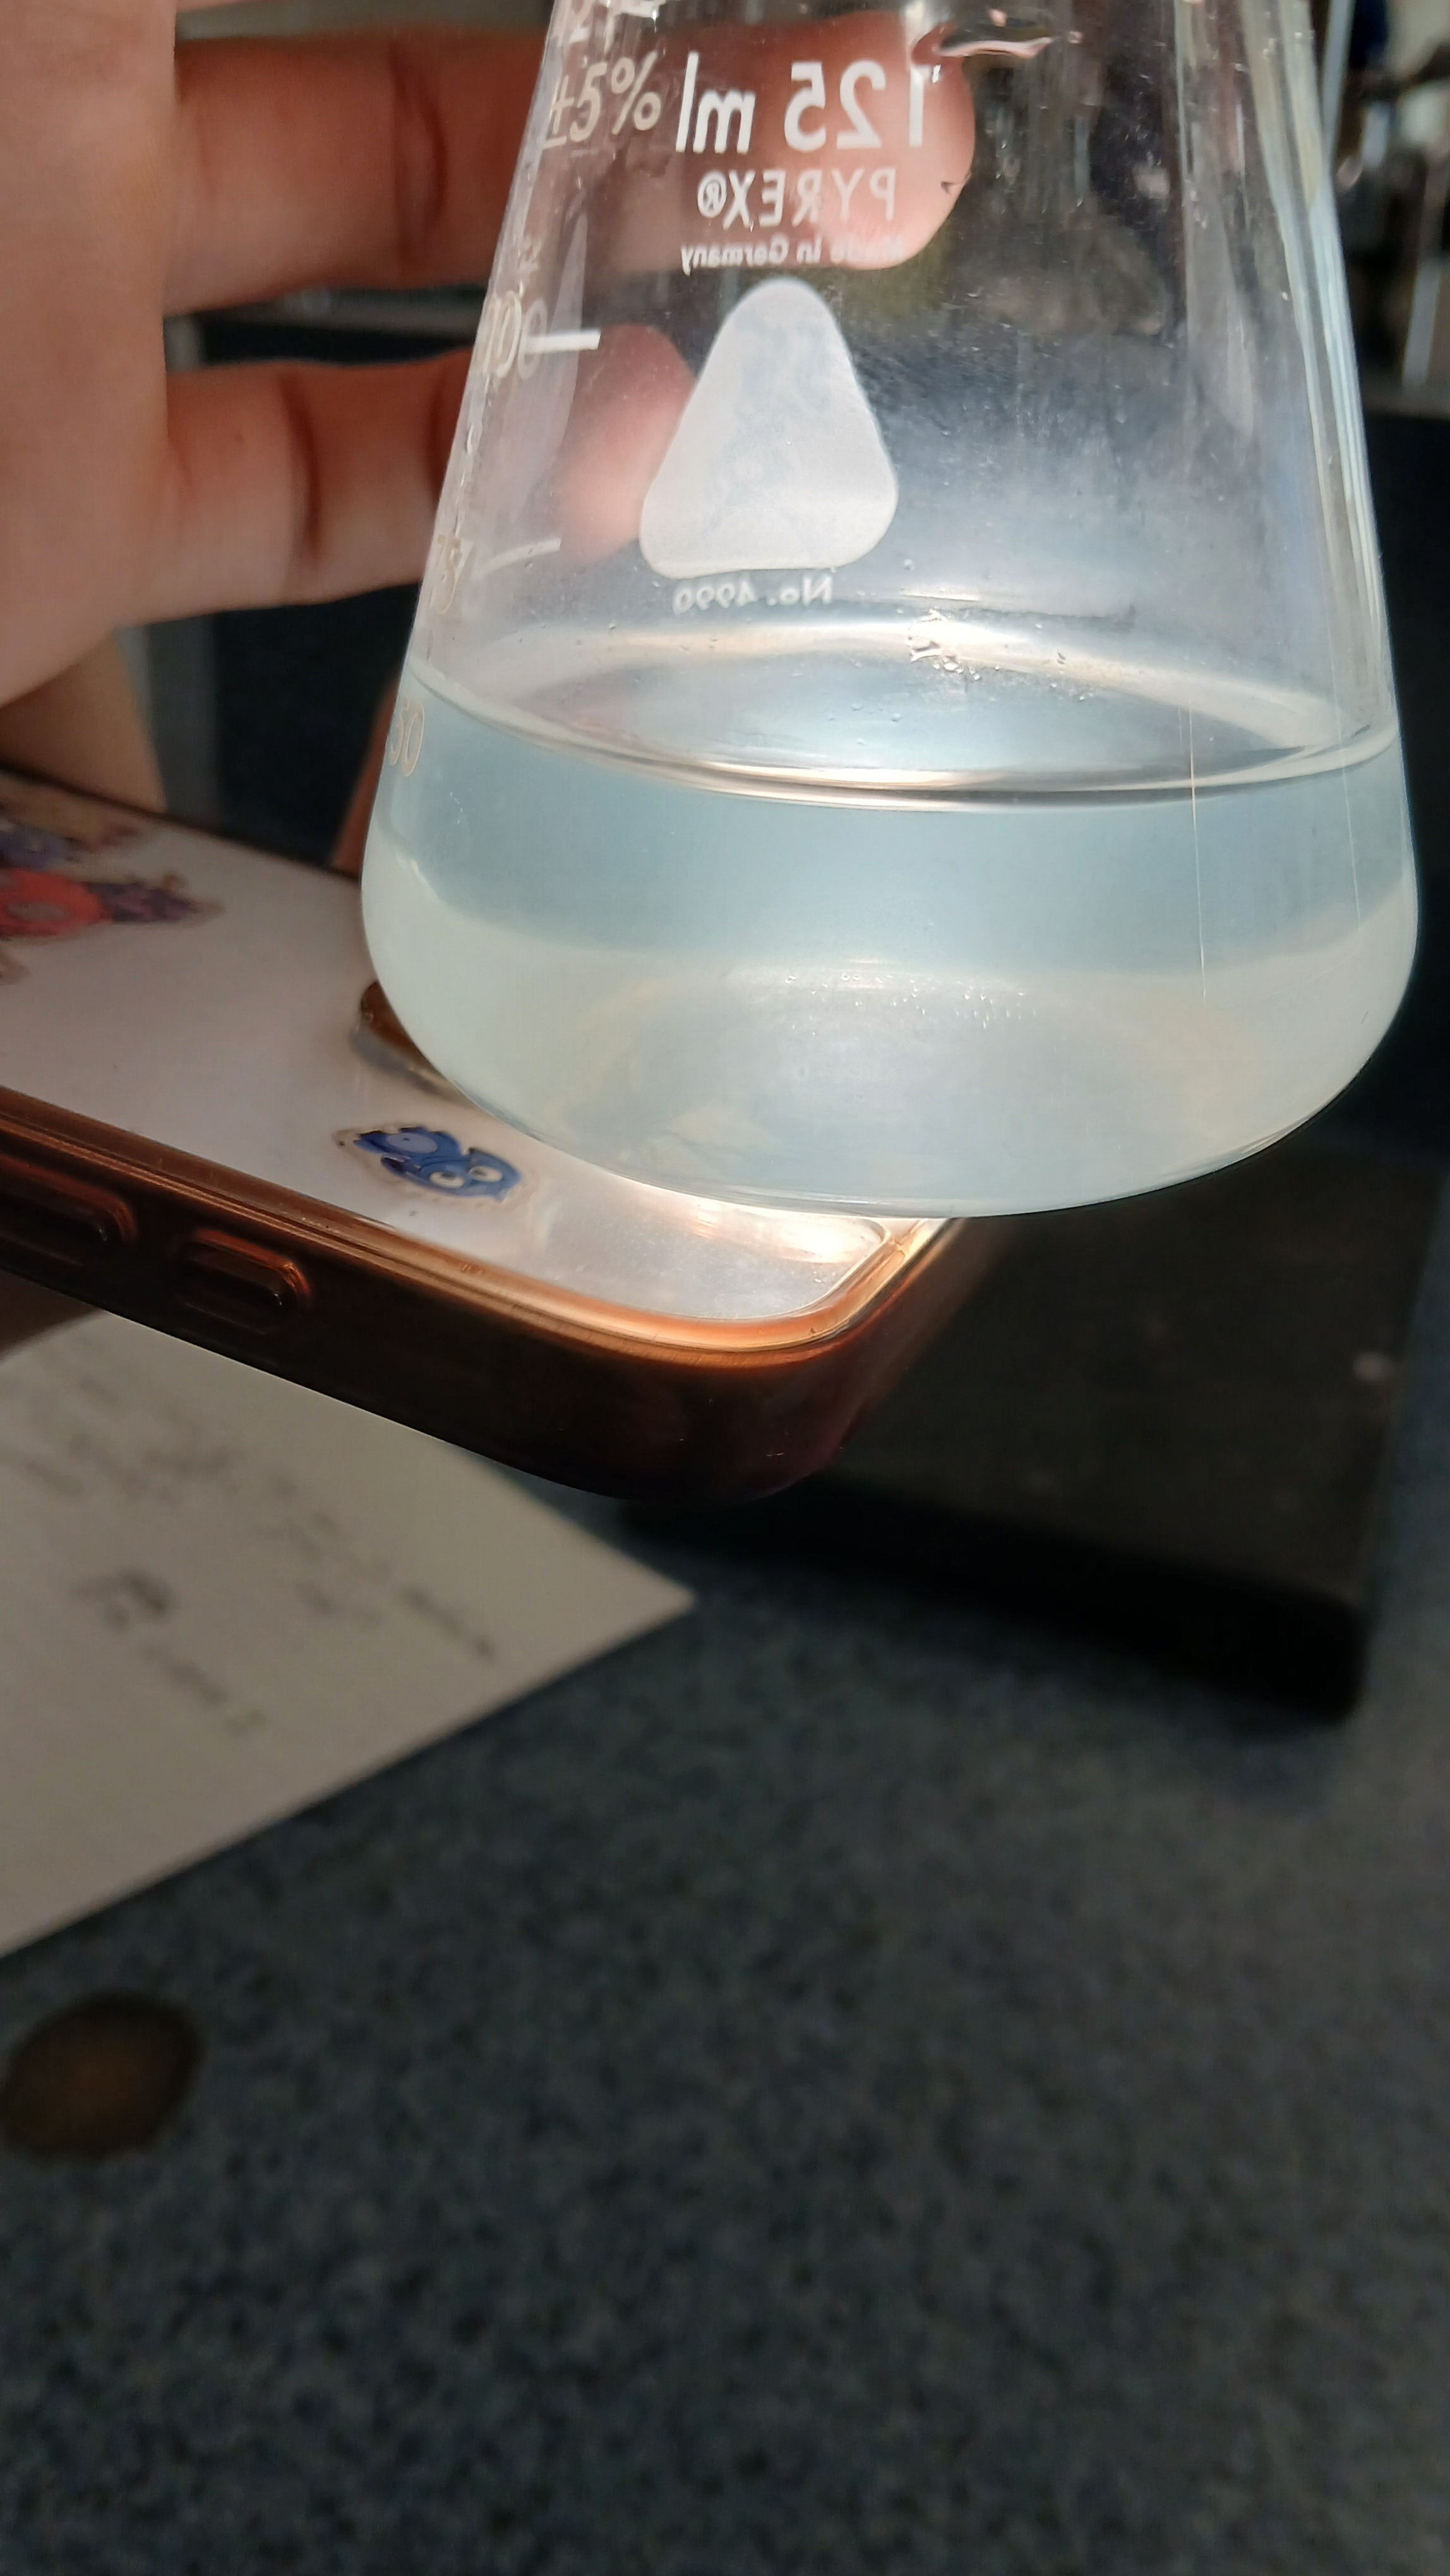
\includegraphics[width=\linewidth]{images/1000053273.jpg}
        \caption{\dv = 5.9 mL.}
    \end{subfigure}
    \hfill
    \begin{subfigure}{0.3\textwidth}
        \centering
        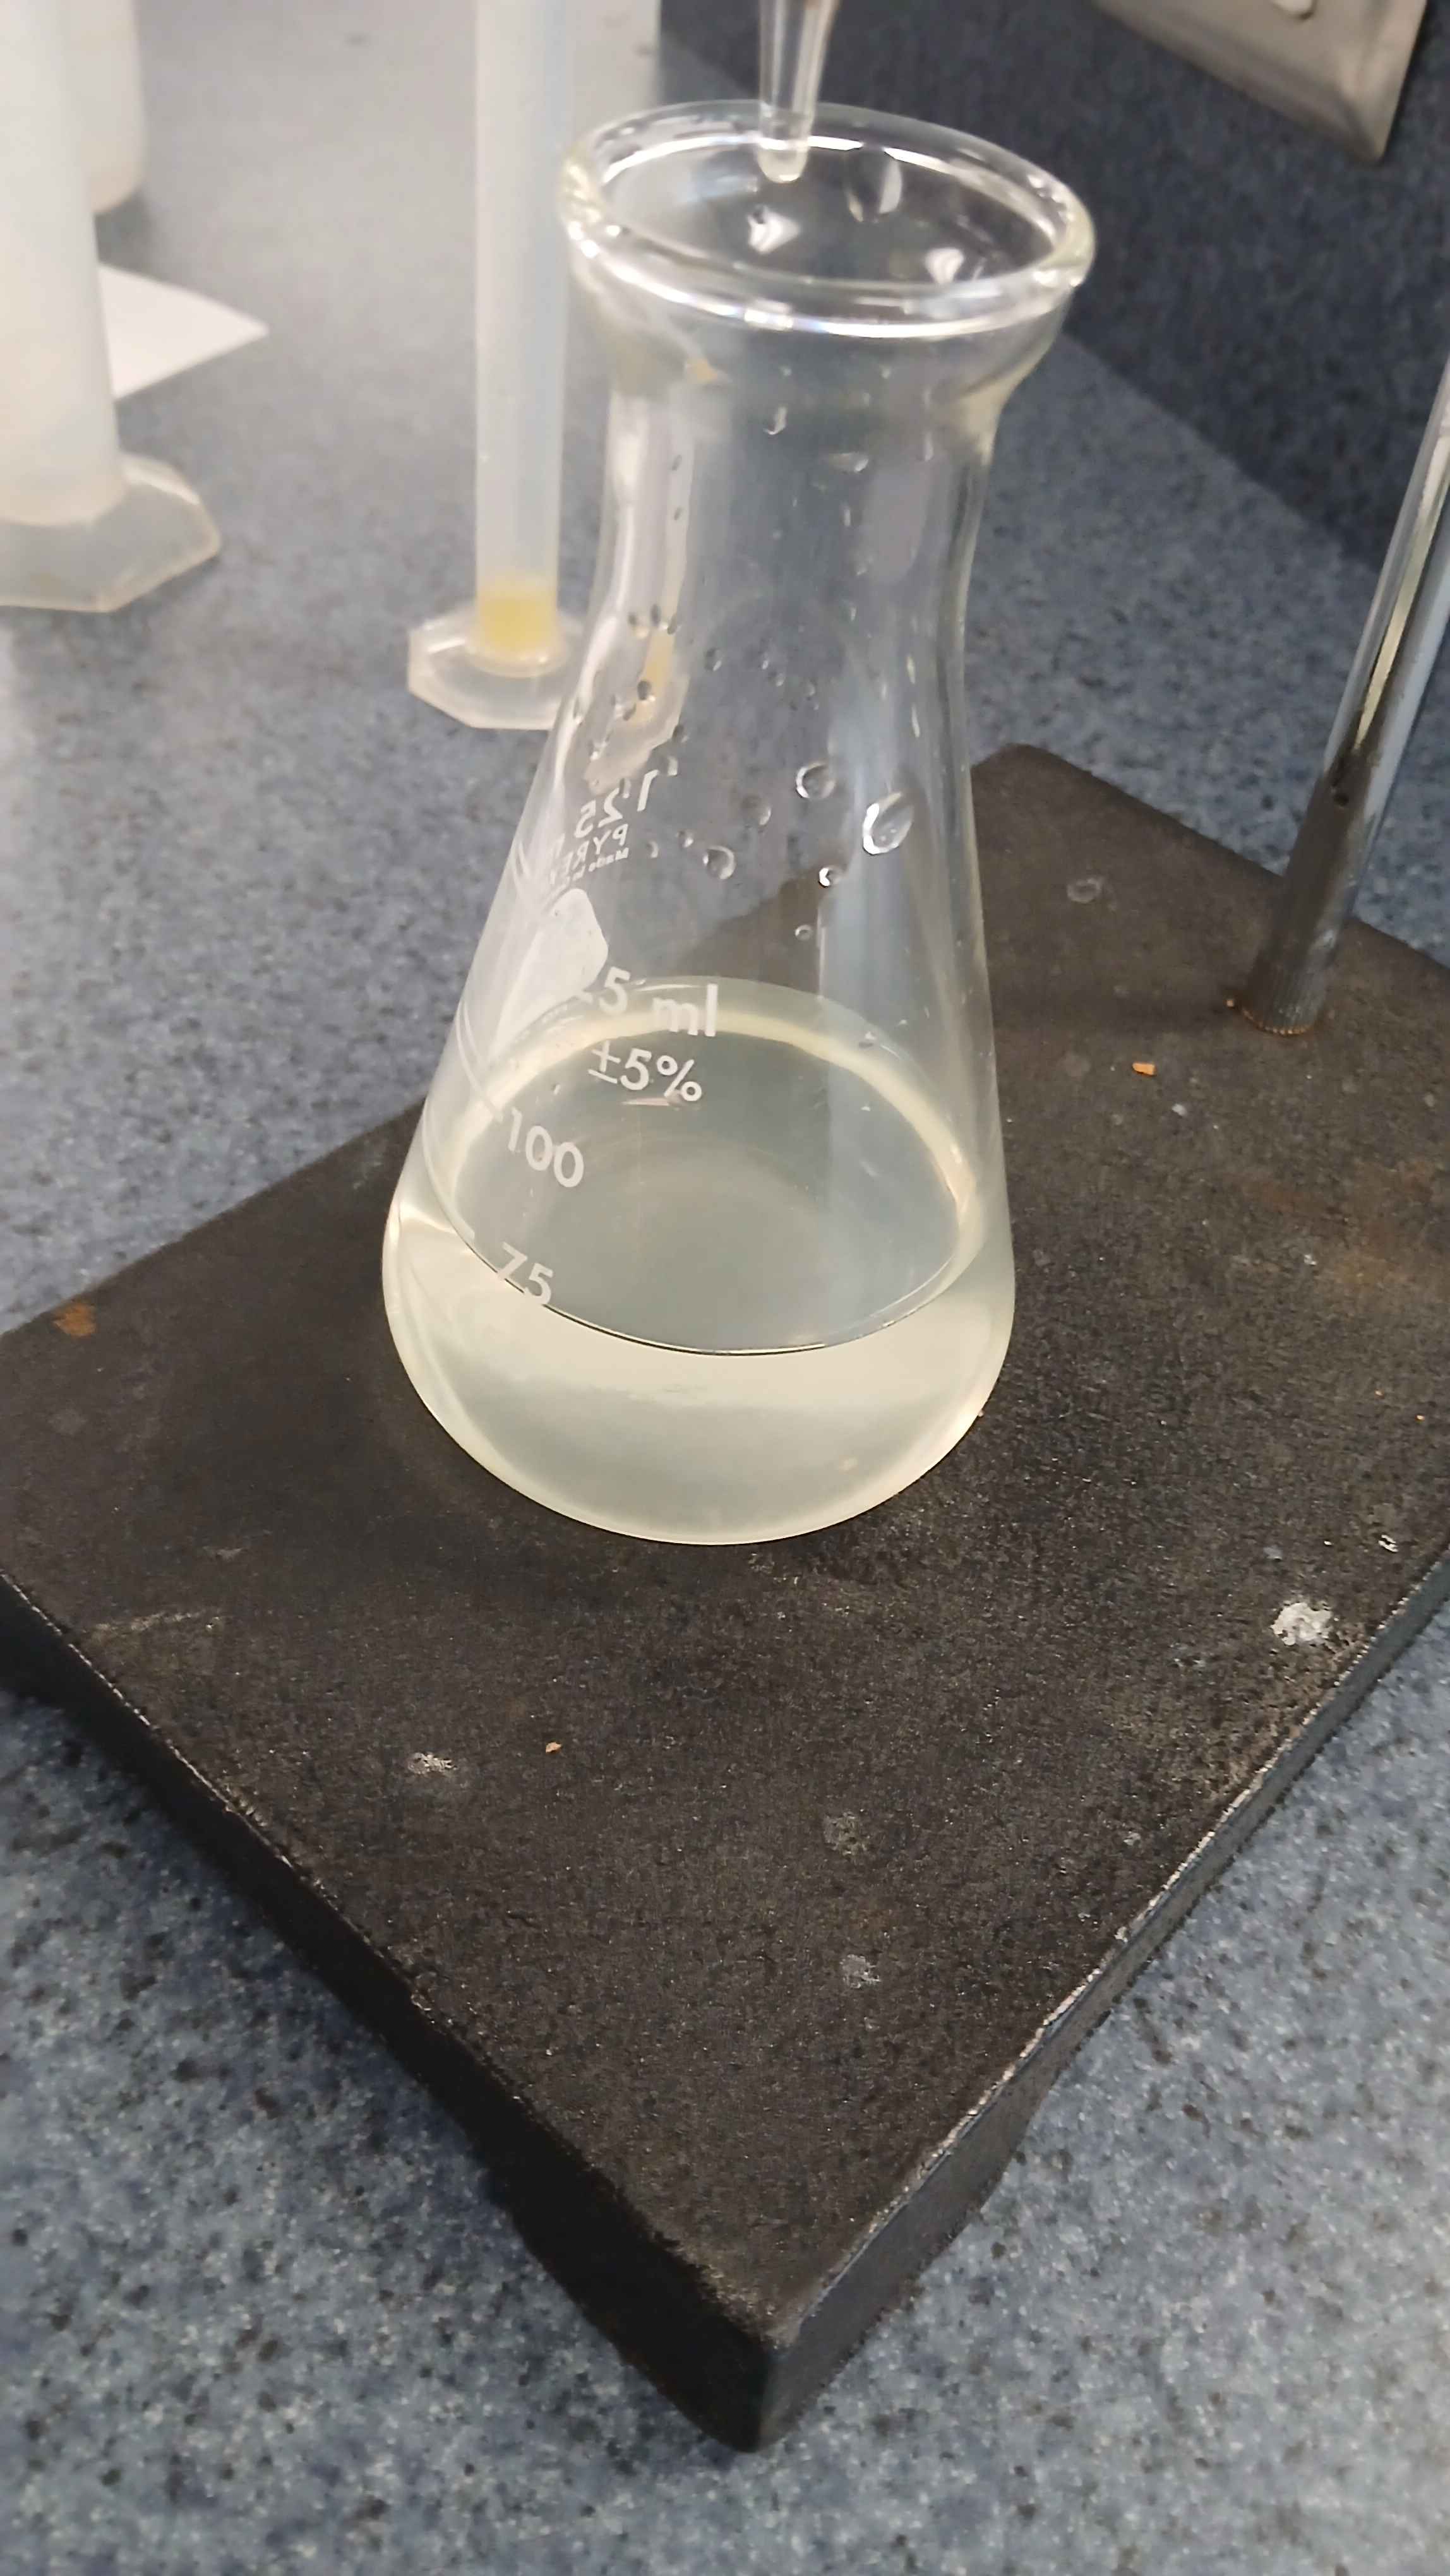
\includegraphics[width=\linewidth]{images/1000053275.jpg}
        \caption{\dv = 12.0 mL.}
    \end{subfigure}
    \hfill
    \begin{subfigure}{0.3\textwidth}
        \centering
        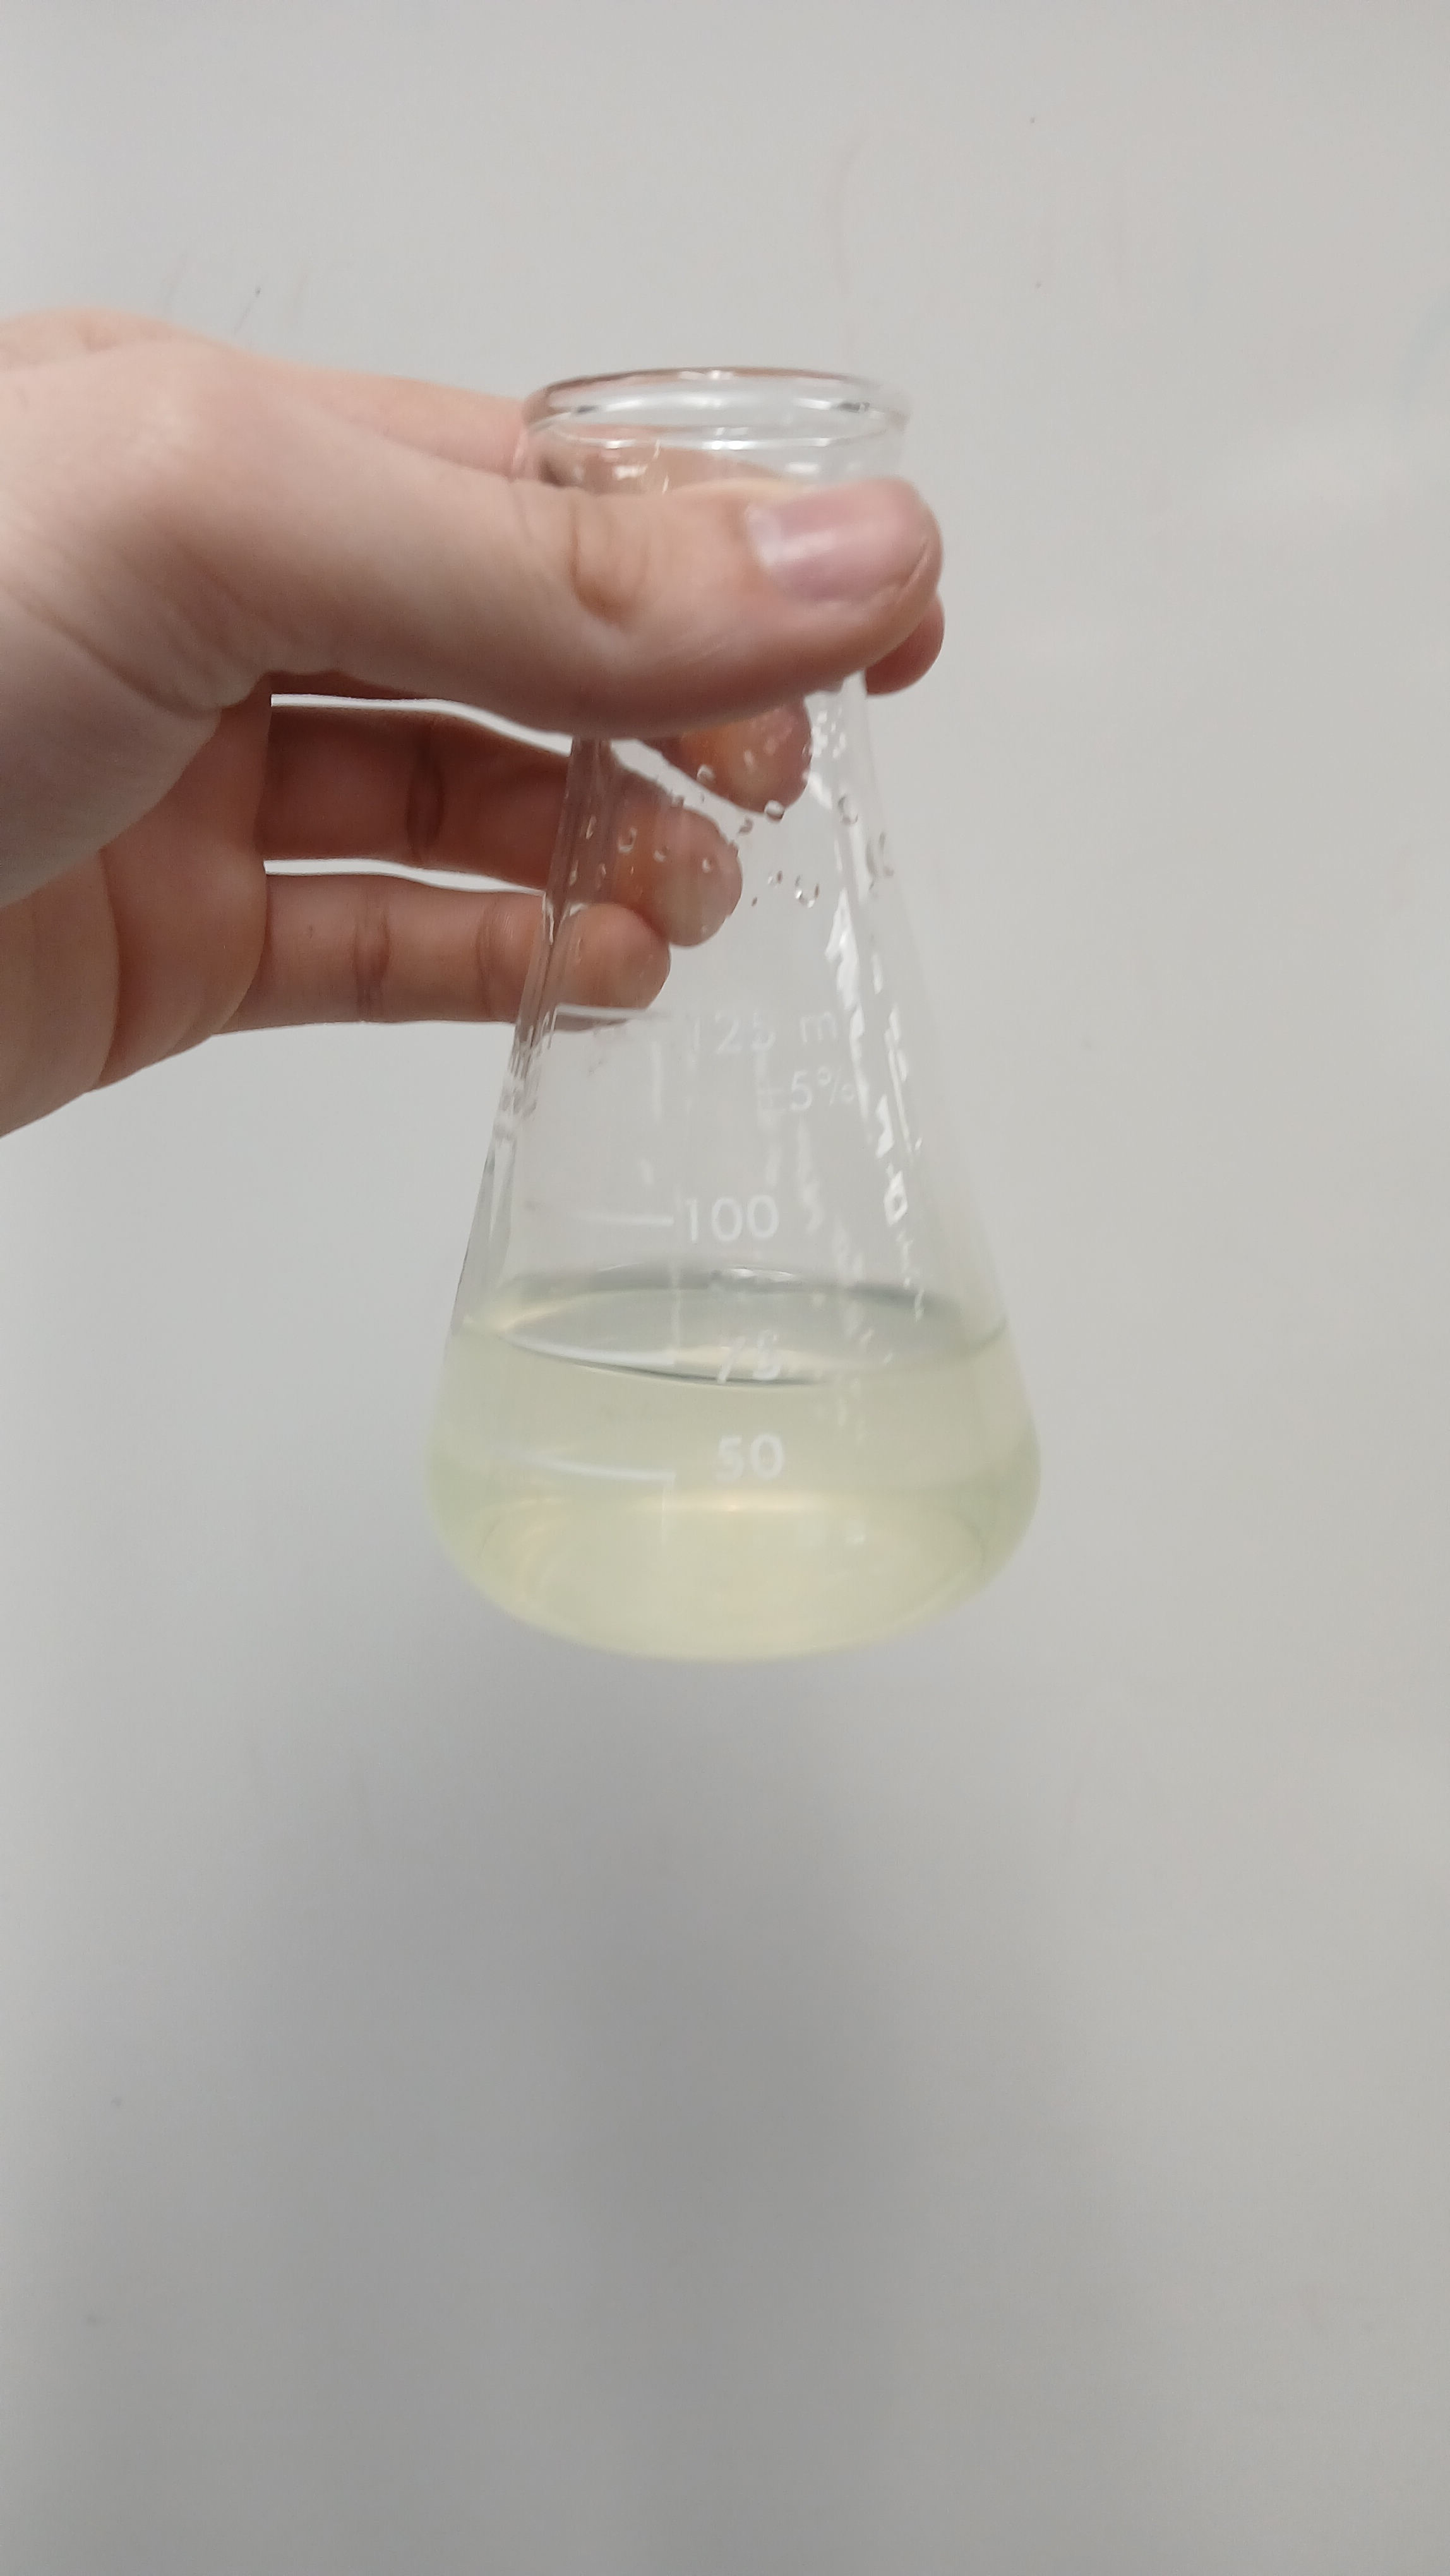
\includegraphics[width=\linewidth]{images/1000053277.jpg}
        \caption{\dv = 14.8 mL.}
    \end{subfigure}
    \caption{Solution at various levels of \dv. Note that the sparkles are not visible in photo a, but were observed in person.}
\end{figure}


\subsection{Alternative Data/Observations}
\begin{table}[H]
    \centering
    
    \begin{minipage}[t]{0.46\textwidth}
        \centering
        \caption{Alternative Data (raw).}
        
        \vspace{0.5em}

        {
            \aboverulesep=0pt
            \belowrulesep=0pt
        \pgfplotstabletypeset[
            col sep=comma,
            string type,
            every head row/.style={
                before row={\midrule},
                after row={\midrule}
            },
            every nth row={1}{before row=\midrule},
            every last row/.style={
                after row={\midrule}
            },
            columns/Parameter/.style={
                column name=\textbf{Parameter},
                column type={|l},
                string type
            },
            columns/Mass (g)/.style={
                column name=\textbf{Mass (g)},
                column type={|c|},
                string type
            }
        ]{data/altdata.csv}
        }
    \end{minipage}
    \hfill
    \begin{minipage}[t]{0.46\textwidth}
        \centering
        \caption{Alternative Data (averages).}
        
        \vspace{0.5em}
        
        {
            \aboverulesep=0pt
            \belowrulesep=0pt
        \pgfplotstabletypeset[
            col sep=comma,
            string type,
            every head row/.style={
                before row={\midrule},
                after row={\midrule}
            },
            every nth row={1}{before row=\midrule},
            every last row/.style={
                after row={\midrule}
            },
            columns/Parameter/.style={
                column name=\textbf{Parameter},
                column type={|l},
                string type
            },
            columns/Mass (g)/.style={
                column name=\textbf{Mass (g)},
                column type={|c|},
                string type
            }
        ]{data/altaverage.csv}
        }
    \end{minipage}
\end{table}

Both solutions started as clear, colourless liquids. When they were mixed, a bright yellow precipitate formed immediately. This was then filtered out and dehydrated in the hot air oven. The dehydrated precipitate appeared as a bright yellow powder. The mass of the precipitate + filter paper was recorded, as well as an an average value for the mass of the filter paper alone.

$$$$

Because we forgot to weigh the filter paper before filtering, we had to use an average value over five filters. Using this value, we can calculate the mass of the precipitate alone:
\begin{align*}
    m_{ppt} &= m_{filter,ppt} - m_{filter,avg} \\
    m_{ppt} &= 2.55g - 2.47g \\
    m_{ppt} &= 0.08g
\end{align*}
